\chapter{Zadania dodatkowe}
	\label{ch:dod}
	
	\section{PID}
		\label{sec:PID}
		
		\begin{figure}[h!]
			\centering
			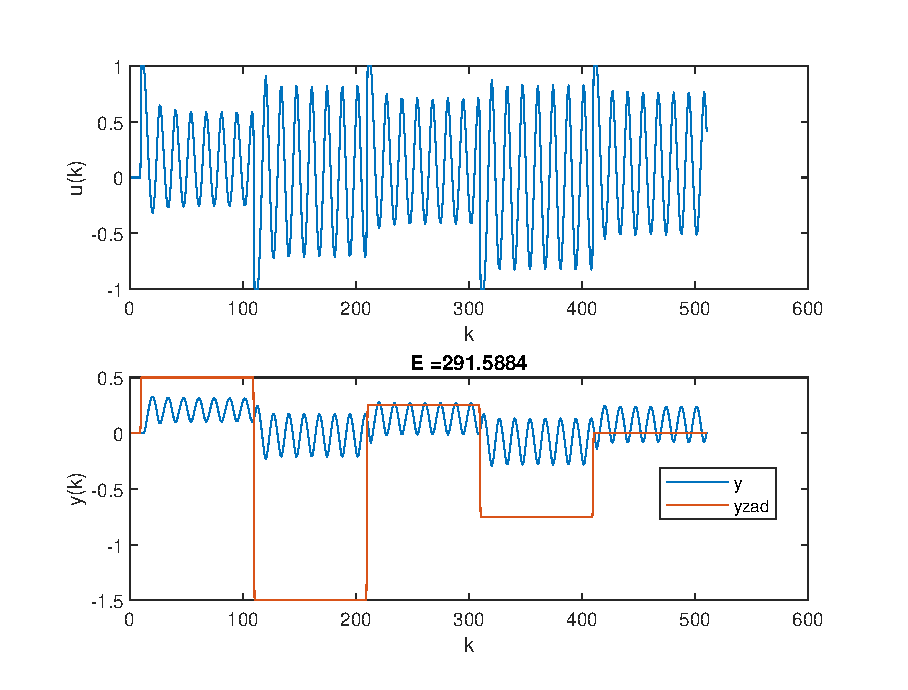
\includegraphics[width=\linewidth]{img/strojeniePID_Kp_4_Ti_duzo_Td_0.eps}
			\caption{Działanie regulatora PID z nastawami Kp = 4, Ti = Inf, Td = 0}
			\label{fig:PID0}
		\end{figure}
		
		\begin{figure}[h!]
			\centering
			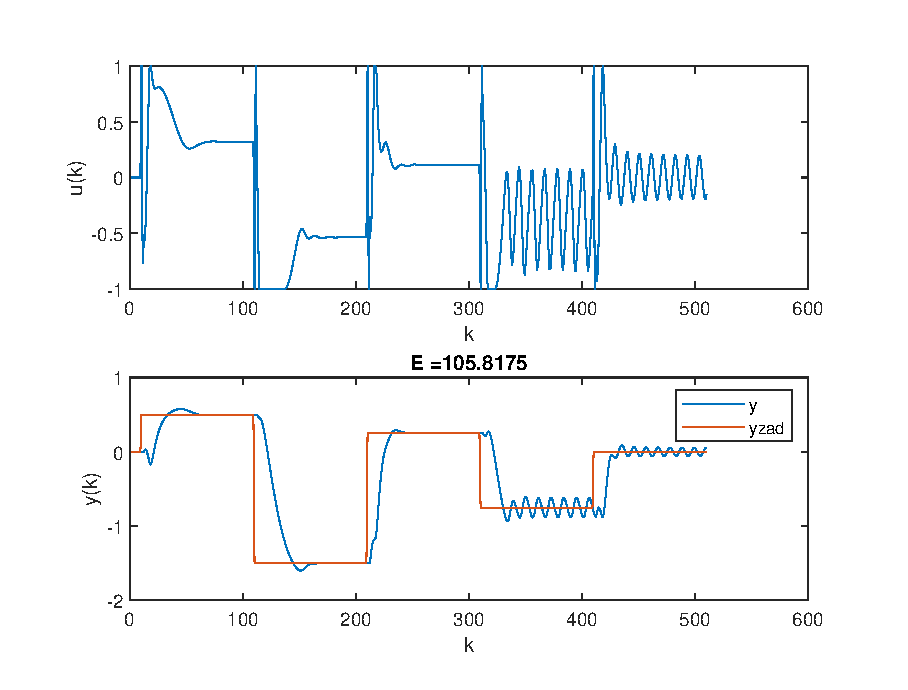
\includegraphics[width=\linewidth]{img/strojeniePID_Ziegler_Nichols.eps}
			\caption{Działanie regulatora PID z nastawami Kp = 2.4, Ti = 6.5, Td = 1.625}
			\label{fig:PID1}
		\end{figure}
		
		
	\section{NO}
		\label{sec:NO}
		
		\begin{figure}[h!]
			\centering
			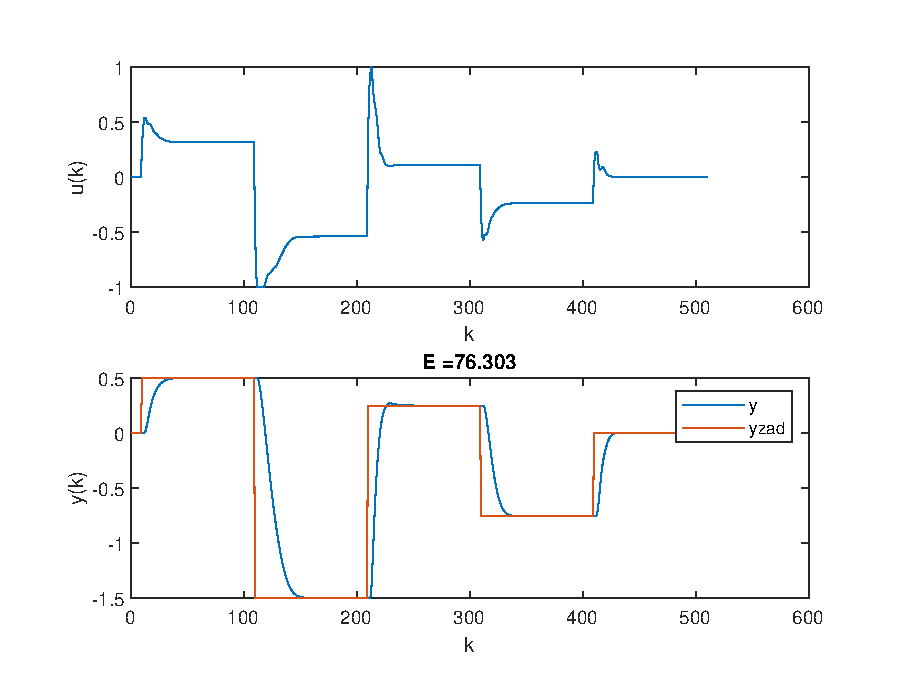
\includegraphics[width=\linewidth]{img/NO.eps}
			\caption{Działanie regulatora NO z nastawami N=20, Nu=2, $\lambda$=2}
			\label{fig:NO}
		\end{figure}